\documentclass{article}
\usepackage[T1]{fontenc}
\usepackage[utf8]{inputenc}
\usepackage[polish]{babel}
\usepackage{ragged2e}
\usepackage{blindtext}
\usepackage{graphicx}
\usepackage{geometry}
\usepackage{setspace}
\usepackage{tabulary}
\usepackage{enumitem}
\usepackage{url}
\usepackage{subfig}
\usepackage{float}
\usepackage[ampersand]{easylist}
%\usepackage{showframe}

\geometry{left=3cm, right=3cm, top=1.5cm, bottom=1.5cm}
\graphicspath{ {./images/} }

\begin{document}
\begin{titlepage}
    \begin{center}

        \vspace*{1cm}
        
        {
            \LARGE
            Akademia Górniczo Hutnicza\\
            \vspace{0.2cm}
            im. Stanisława Staszica w Krakowie
        }

        \vspace{0.5cm}

        \begin{figure}[h]
            \centering
            
\includegraphics[width=\textwidth]{logo.png}
        \end{figure}

        \vspace{0.5cm}

        {
            \LARGE
            Wydział Inżynierii Metali i Informatyki Przemysłowej\\
            \vspace{0.2cm}
            Katedra Informatyki Stosowanej i Modelowania
        }

        \vspace{0.5cm}

        {
            \LARGE
            Praca Dyplomowa Inżynierska
        }

        \vspace{0.5cm}

        {
            \Large
            \textbf{,,Interaktywne przetwarzanie obrazów mikroskopowych\\
            związanych z oceną adhezji składników komórkowych''}
        }

        \vspace{0.5cm}

        {
            \Large
            \textbf{,,Interactive processing of microscopic images\\
            related to evaluation adhesion of cellular components''}
        }

        \vfill

        \begin{flushleft}
        {
            \Large
            \begin{tabular}{ l l c }
                autor: & Konrad Lenart\\
                kierunek: & Inżynieria Obliczeniowa\\
                opiekun pracy: & dr hab. Magdalena Kopernik
            \end{tabular}
        }
        \end{flushleft}

        \vspace{0.5cm}

        {
            \Large
            Kraków, 2020
        }

        \vspace{1cm}

    \end{center}
\end{titlepage}

\setstretch{2.5}
    \newpage
    {
        \Large
        \justifying
        Uprzedzony o odpowiedzialności karnej na podstawie art. 115 ust. 1 i 2 ustawy z dnia 4 lutego
        1994 r. o prawie autorskim i prawach pokrewnych (tj. Dz.U. z 2006 r. Nr 90, poz. 631 z późn.
        zm.): „Kto przywłaszcza sobie autorstwo albo wprowadza w błąd co do autorstwa całości lub
        części cudzego utworu albo artystycznego wykonania, podlega grzywnie, karze ograniczenia
        wolności albo pozbawienia wolności do lat 3. Tej samej karze podlega, kto rozpowszechnia bez
        podania nazwiska lub pseudonimu twórcy cudzy utwór w wersji oryginalnej albo w postaci
        opracowania, artystyczne wykonanie albo publicznie zniekształca taki utwór, artystyczne
        wykonanie, fonogram, wideogram lub nadanie.”, a także uprzedzony o odpowiedzialności
        dyscyplinarnej na podstawie art. 211 ust. 1 ustawy z dnia 27 lipca 2005 r. Prawo o szkolnictwie
        wyższym (tj. Dz. U. z 2012 r. poz. 572, z późn. zm.) „Za naruszenie przepisów obowiązujących
        w uczelni oraz za czyny uchybiające godności studenta student ponosi odpowiedzialność
        dyscyplinarną przed komisją dyscyplinarną albo przed sądem koleżeńskim samorządu
        studenckiego, zwanym dalej „sądem koleżeńskim”, oświadczam, że niniejszą pracę
        dyplomową wykonałem osobiście, samodzielnie, i że nie korzystałem ze źródeł innych niż
        wymienione w pracy.
    }

    \vfill

    \begin{center}
        {
            \Large
            \setstretch{1.0}
            \setlength{\tabcolsep}{2em}
            \begin{tabulary}{0.75\textwidth}{ c c c }
                Kraków, dnia........................ && ................................\\
                (miejscowość)& & (podpis)\\
            \end{tabulary}
        }
    \end{center}
    
    \newpage
    \begin{center}
        {
            \Large
            \setstretch{1.0}
            \tableofcontents
        }
    \end{center}
    \newpage
    
    \section{Wstęp}
    \setstretch{1.5}
    {
        \Large
        \justifying
        \quad 
        Każdy dzień to nowy rekord postępu dla całej cywilizacji technicznej.
        Szybkość z jaką pojawiają się nowe technologie stale rośnie.
        Nikogo nie dziwi już ile ludzkość potrafi dokonać w ciągu dwudziestu czterech godzin.
        Obecny trend rozwoju zawdzięczamy pojawieniu się komputerów.
        Komputery zastąpiły ludzi w wielu czynnościach, stworzyły także nowe miejsca pracy.
        Wyreczają nas w skomplikowanych obliczeniach, pozwalają testować systemy bezpieczeństwa w samochodach bez konieczności ich niszczenia, nauczyliśmy je nawet pilotować olbrzymie samoloty.
        Każdy z nas nosi w kieszeni większą moc obliczeniową niż komputery obecne na statkach kosmicznych, które lądowały na księżycu w ramach programu Apollo.
        Zaprzęgnięcie komputerów do automatyzacji pracy, którą ludzie do tej pory wykonywali ręcznie zaoszczędza nam sporo czasu.
        Charakter tej pracy jest analogiczny - zastąpienie ludzi w mozolej, ręcznej ocenie adhezji składników komórkowych -
        automatycznym procesem, który przez człowieka będzie tylko nadzorowany.
    }
    
    \vspace{1cm}
    \setstretch{1.5}
    {
        \Large
        \justifying
        Jedną z najważniejszych dziedzin, w której komputery znalazły zastosowanie jest medycyna.
        Postęp w tej dziedzinie ratuje każdego dnia miliony istnień na całym świecie.
        W niniejszej pracy podjęto próbę oceny adhezji składników komórkowych wykorzystując do tego analizę i przetwarzanie obrazów cyfrowych pochodzących z mikroskopu.
        Z pomocą odpowiednich algorytmów zliczone zostają obiekty widoczne na zdjęciu.
        Następnie bazując na faktach o składnikach komórkowych krwii obiekty zostają zakwalifikowane jako komórka krwii lub odrzucone.
    }

    \vspace{1cm}
    \setstretch{1.5}
    {
        \Large
        \justifying
        Założeniem pracy było stworzenie łatwej w obsłudze biblioteki napisanej w języku C++.
        Biblioteka napisana została w taki sposób, aby z łatwością można było dołączyć ją do istniejących projektów w środowisku Visual Studio.
        Cele poboczne pracy to stworzenie interfejsu użytkownika w celu zaprezentowania funkcjonalności bibilioteki.
        Do tego celu wykorzystana została aplikacja na komputery osobiste z wykorzystaniem .NET Framework 4.7.2.
        Dokładny opis biblioteki jak i interfejsu użytkownika ma miejsce w rozdziale drugim.
        Po części teoretycznej traktującej o wszystkich wykorzystanych w programie zagadnieniach związanych z analizą i przetwarzaniem obrazów cyfrowych. 
    }

    \vfill

    \newpage
    \section{Cele i założenia}
        \subsection{Cel główny}
        \setstretch{1.5}
        {
            \Large
            \justifying
            \quad
            Celem głównym było stworzenie biblioteki zajmującej się analizą i przetwarzaniem obrazów cyfrowych.
            Biblioteka ma za zadanie ocenę adhezji komórek krwi widocznych na obrazach pochodzących z mikroskopu.
            Podczas pracy nad biblioteką utrzymywany był kontakt z osobami, które będą z niej korzystać.
            Biblioteka napisana została w taki sposób, aby dostosować jej funkcjonalności do istniejącej już metodologii.
            Ma również drugie zadanie - ułatwić oraz usprawnić pracę ludzi.
            Dzięki temu analiza obrazów niosących informacje na temat krwi pozowli zaoszczędzić znaczącą ilość czasu.
        }
        \subsection {Cel poboczny}
        \setstretch{1.5}
        {
            \Large
            \justifying
            \quad
            Celem pobocznym było stworzenie interatywnej aplikacji okienkowej, w której zaprezentowane zostało działanie biblioteki.
            Aplikacja służy zaprezentowaniu procesów zachodzących podczas analizy i przetwarzania obrazów cyfrowych.
            Pozwala również na interakcje z procesem, jego zmiane, zatrzymanie, dostosowanie parametrów oraz podgląd tego co się dzieje w czasie rzeczywistym.
            Do tego celu zostały wykorzystane następujące technologie: C++/CLI, C\#, Windows Presentation Foundation oraz .NET Framework 4.7.2.
        }
        \subsection{Założenia}
        \setstretch{1.5}
        {
            \Large
            \justifying
            \quad
            Głównym założeniem tworzonego oprogramowania było stworzenie biblioteki w taki sposób, aby osoby z niej korzystające z łatwością mogły dodac ją do swoich projektów w środowisku Visual Studio 2019.
            Funkcjonalności jakie niesie ze sobą nie skupiają się wyłącznie na analizie i przetwarzaniu obrazów cyfrowych.
            Biblioteka dba również o to, aby struktura folderów była w należytym stanie na podstawie głownego folderu.
            Główny folder powinien gromadzić kolejne foldery tak zwane eksperymenty, gdzie przez eksperyment rozumiemy folder, w którym znajdują się dane pochodzące z mikroskopu.
            W każdym z takich folderów dodane zostają odpowiednie pliki odpowiedzalne za ustawienia.
            Jeżeli dany eksperyment posiada juz plik ustawień, jest to jasny sygnał dla programu, że nie należy dodawac kolejnego.
        }

        \vspace{0.5cm}
        \setstretch{1.5}
        \subsection{Podstawowe funkcje biblioteki}
        {
            \Large
            \quad
            \begin{enumerate}
                \item Analiza drzewa folderów,
                \item Zliczanie komórek krwi na obrazach cyforwych,
                \item Zapis wyniku pracy algorytmu zliczającego ilość komórek krwii w ramach eksperymentu do pliku.
            \end{enumerate}
        }

        \vspace{0.5cm}
        \setstretch{1.5}
        \subsection{Podstawowe funkcje aplikacji okienkowej}
        {
            \Large
            \quad
            \begin{enumerate}
                \item Możliwość zmiany ustawień przetwarzania obrazów w ramach eksperymentu --> GUI,
                \item Możliwość dostosowania parametrów dla każdego z obrazów w czasie rzeczywistym --> GUI,
                \item Możliwość śledzenia algorytmu w czasie rzeczywistym --> GUI,
                \item Możliwość podglądu postępu przetwarzania obrazów --> GUI,
                \item Wyświetlanie histogramu w ramach eksperymentu --> GUI,
                \item Możliwość wyświetlania czasu przetwarzania danego obrazu --> GUI,
            \end{enumerate}
        }

        \vspace{1cm}
        \setstretch{1.5}
        \subsection{Rekomendacje}
        {
            \Large
            \justifying
            \quad
            Użytkownikom oprogramowania rekomenduje sie wykorzystywanie biblioteki na systemie operacyjnym Windows 10 w projektach budowanych z wykorzystaniem MSBuild (Microsoft Build Engine) w konfiguracji 64-bitowej. \cite{msdocsmsbuild}
        }
    \newpage
    \section{Część teoretyczna}
        \subsection{Adhezja}
        {
            \Large
            \justifying
            \quad
            //todo:
        }
        \subsection{Rozszerzenie TIFF}
        {
            \Large
            \justifying
            \quad
            TIFF - \textit{Tag Image File Format} jest to format plików służący do przechowywania obrazów rastrowych.
            TIFF ma bardzo szerokie zastosowania, od urzadzeń służących do skanowania czy wysyłania faksów, do analizy i przetwarzania obrazów cyfrowych.
            Format stworzony przez \textit{Aldus Corporation}, nieistniejącego już dzisiaj przedsiębiorstwa przejętego w 1994 przez \textit{Adobe}.
            TIFF jest elastycznym i adaptatywnym typem plików służącym do przechowywania zdjęć bez utraty ich jakości.
            Dzięki temu, że przechowywane dane nie tracą jakości, TIFF jest używany do archiwizacji zdjęć, ponieważ w przeciwieństwie do rozszerzenia JPEG,
            TIFF może być zmieniany i zapisywany wielokrotnie bez utraty jakości obrazu.
            Rozszerzenie to niesie ze sobą możliwość pracy zarówno wykorzystując kolory z palety RGB czy też monochromatyczne.
            Jest to bardzo użyteczny format, szczególnie w kontekscie analizy i przetwarzania obrazów cyfrowych. \cite{encyclopediaofgraphicsfileformats}
        }
        \subsection{Binaryzacja}
        {
            \Large
            \justifying
            \quad
            Binaryzacja - służy do stworzenia nowego obrazu na podstawie innego w taki sposób, aby zaznaczyć interesujący nas fragment na czarno(białe tło)
            lub na biało(czarne tło). Jak sama nazwa wskazuje wartości w nowym obrazie są 0 lub 1. Dzięki binaryzacji jesteśmy w stanie przetwarzać obraz
            tylko dla fragmentów zaznaczonych w procesie binaryzacji. Binaryzację można przeprowadzać na przykład na podstawie wartości kolorów w poszczególnych
            macierzach RGB. Na przykład: 
            jeżeli \(czerwony > 150\) i \(zielony > 200\) i \(niebieski < 122\) to wartość danego pixela w nowym obrazie równa się 1.
            Teraz wystarczy zastosować to dla każdego piksela w obrazie wejściowym i naszym obrazem wyjściowym staje się obraz o tym samym rozmiarze
            z zaznaczonym na czarno obszarem, gdzie macierze RGB miały wartości \(czerwony > 150\) i \(zielony > 200\) i \(niebieski < 122\).
            Tak więc, gdy dokonamy już binaryzacji jesteśmy gotowi do kolejnych działań.
            Takich jak na przykład etykietowanie, erozja, dylatacja, otwarcie, zamkniecie czy innego rodzaju operacje morfologiczne. \cite{digitalimageprocessing}
        }
        \subsection{Element Strukturalny}
        {
            \Large
            \justifying
            \quad
            Element Strukturalny - operacje morfologiczne opierają się na elemencie strukturalnym.
            Przez element strukturalny należy rozumieć ruchome okno, które przykładane jest do każdego piksela w obrazie.
            Na podstawie wartości w sąsiedztwie wykonywane są pewne operacje.
            Po przyłożeniu punktu centralnego do piksela, sprawdzana jest wartość tego piksela.
            Jeżeli wartość ta jest równa \(1\) to zazwyczaj oznacza to aktywację.
            Na przykład zamalowanie odpowiednich sąsiadów danego piksela zgodnie z tym, jak wygląda element strukturalny.
            Każdy z punktów elementu strukturalnego ma odpowiednią wartość.
            Punkt centralny punktu strukturalnego to miejsce, które przykłada się do kolejnych pikseli w obrazie binarnym.
            W zależności od operacji morfologicznej, która jest przeprowadzana.
            Pozostałe piksele przyjmują jakąś wartości \(0\) lub \(1\).
            Przykłady elementów strukturalnych (czerwonym kolorem zaznaczono punkty centralne, szarym wartość \(1\), białym wartość \(0\)):
        }
        \begin{figure}[H]
            \captionsetup{margin=1.5cm}
            \centering
            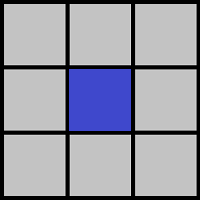
\includegraphics[width=120px]{element_strukturalny_1.png}
            \caption
            {
                (\textit{Opracowanie własne}) Przykład elementu strukturalnego o rozmiarze \(3 \times 3\) z punktem m w środku.
                Wszystkie piksele elementu strukturalnego posiadają wartość równą 1.
            }
        \end{figure}
        \begin{figure}[H]
            \captionsetup{margin=1.5cm}
            \centering
            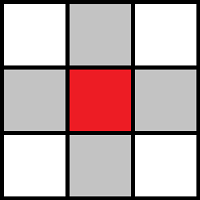
\includegraphics[width=120px]{element_strukturalny_2.png}
            \caption
            {
                (\textit{Opracowanie własne}) Przykład elementu strukturalnego o rozmiarze \(3 \times 3\) z punktem centralnym w środku.
                Lewy dolny, lewy górny, prawy dolny oraz prawy górny piksel posiada wartość 0.
            }
        \end{figure}
        \begin{figure}[H]
            \captionsetup{margin=1.5cm}
            \centering
            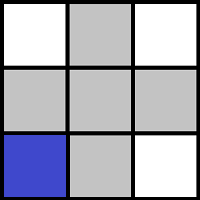
\includegraphics[width=120px]{element_strukturalny_3.png}
            \caption
            {
                (\textit{Opracowanie własne}) Przykład elementu strukturalnego o rozmiarze \(3 \times 3\) z punktem centralnym w lewym dolnym rogu.
                Lewy górny, prawy górny oraz prawy dolny piksel posiada wartość 0.
            }
        \end{figure}
        \begin{figure}[H]
            \captionsetup{margin=1.5cm}
            \centering
            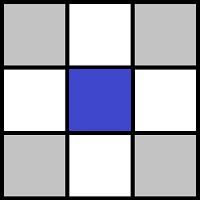
\includegraphics[width=120px]{element_strukturalny_4.png}
            \caption
            {
                (\textit{Opracowanie własne}) Przykład elementu strukturalnego o rozmiarze \(3 \times 3\) z punktem centralnym w środku.
                Lewy środkowy, prawy środkowy, dolny środkowy oraz górny środkowy piksel posiada wartość 0.
            }
        \end{figure}
        \begin{figure}[H]
            \captionsetup{margin=1.5cm}
            \centering
            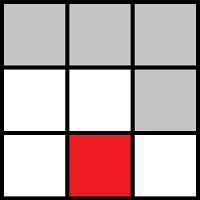
\includegraphics[width=120px]{element_strukturalny_5.png}
            \caption
            {
                (\textit{Opracowanie własne}) Przykład elementu strukturalnego o rozmiarze \(3 \times 3\) z punktem centralnym w dolnym środkowym pikselu.
                Lewy dolny, lewy środkowy, środkowy oraz prawy dolny piksel mają wartość równą 0.
            }
        \end{figure}
        \subsection{Sąsiedztwo}
        {
            \Large
            \justifying
            \quad
            Sąsiedztwo - jest to sposób w jaki zdefiniowane jest otoczenie danego piksela.
            Wyróżnia się dwa głowne sąsiedztwa: Moore'a oraz Von Neumanna. Jak pokazano na Rysunku \ref{fig:Neighbourhood}:
        }
        \begin{figure}[H]
            \centering
            \subfloat[\centering Sąsiedztwo Moore'a]{{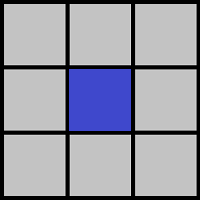
\includegraphics[width=5cm]{element_strukturalny_1.png}}}
            \qquad
            \subfloat[\centering Sąsiedztwo Von Neumanna]{{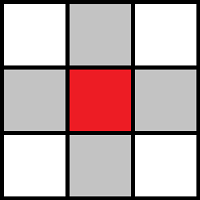
\includegraphics[width=5cm]{element_strukturalny_2.png}}}
            \caption{(\textit{Opracowanie własne}) Sąsiedztwa}
            \label{fig:Neighbourhood}
        \end{figure}
        \subsection{Erozja}
        {
            \Large
            \justifying
            \quad
            Erozja - czyli zwężanie.
            Przyłożenie elementu strukturalnego do każdego piksela \(p_{ij}\) na obrazie w celu sprawdzenia czy choć jeden piksel z sąsiedztwa \(p_{ij}\) ma wartość równą zero.
            Jeżeli tak - punkt centralny również przyjmuje wartość 0. W przeciwnym przypadku wartość pozostaje bez zmian.
        }
        \begin{figure}[H]
            \centering
            \subfloat[\centering Element strukturalny użyty w operacji]{{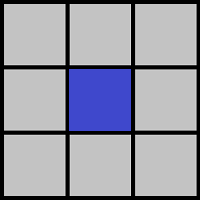
\includegraphics[width=5cm]{element_strukturalny_1.png}}}
            \qquad
            \subfloat[\centering Stan przed erozją elementem strukturalnym]{{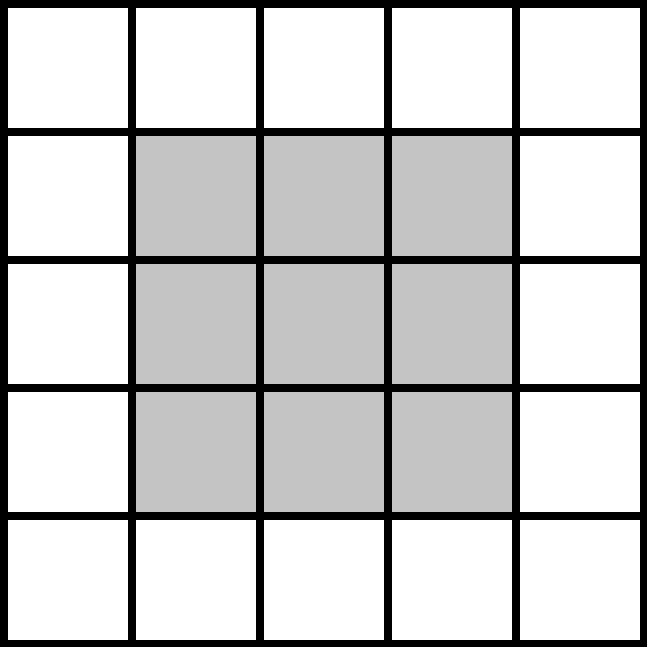
\includegraphics[width=5cm]{przed_erozja.png}}}
            \qquad
            \subfloat[\centering Stan po erozji elementem strukturalnym]{{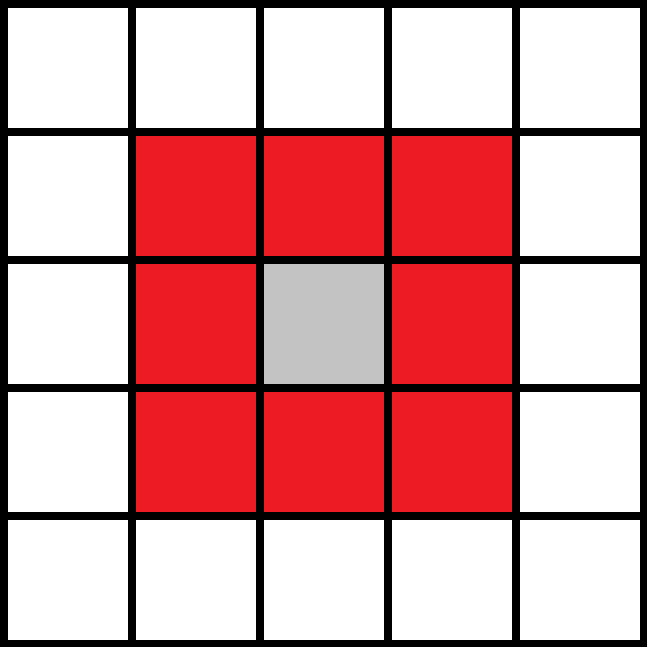
\includegraphics[width=5cm]{po_erozji.png}}}
            \caption
            {
                (\textit{Opracowanie własne}) Erozja (Czerwonym kolorem zaznaczono piksele, które zmieniły wartości z 1 na 0)
            }
        \end{figure}
        \subsection{Dylatacja}
        {
            \Large
            \justifying
            \quad
            Dylatacja - czyli rozszerzanie.
            Przyłożenie elementu strukturalnego do każdego piksela \(p_{ij}\) na obrazie w celu sprawdzenia czy choć jeden z piksel z sąsiedztwa \(p_{ij}\) ma wartość równą jeden.
            Jeżeli tak - punkt centralny również przyjmuje wartość 1. W przeciwnym wypadku wartość nie ulega zmianie.
        }
        \begin{figure}[H]
            \centering
            \subfloat[\centering Element strukturalny użyty w operacji]{{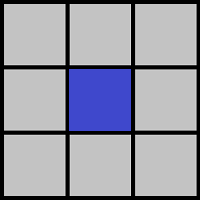
\includegraphics[width=5cm]{element_strukturalny_1.png}}}
            \qquad
            \subfloat[\centering Stan przed dylatacją elementem strukturalnym]{{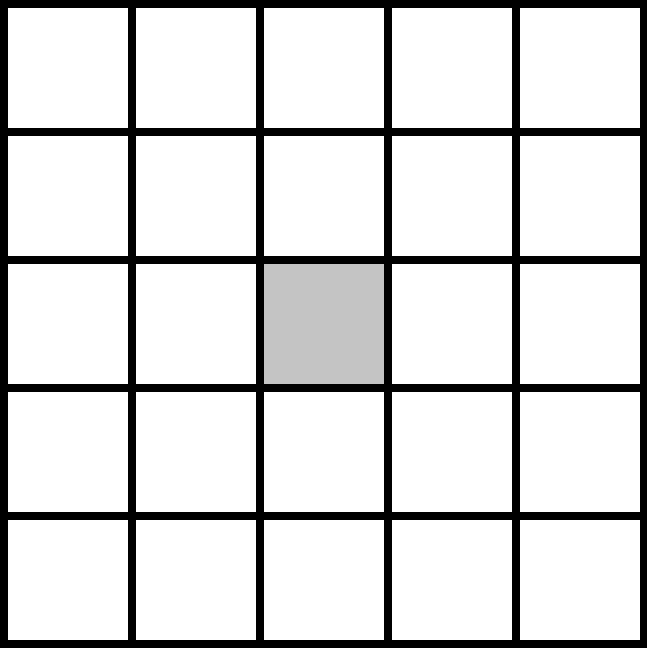
\includegraphics[width=5cm]{przed_dylatacja.png}}}
            \qquad
            \subfloat[\centering Stan po dylatacji elementem strukturalnym]{{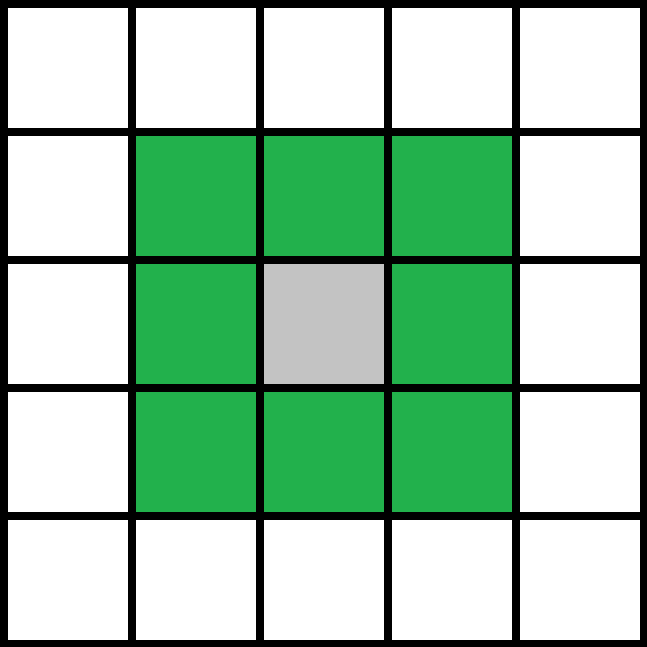
\includegraphics[width=5cm]{po_dylatacji.png}}}
            \caption{(\textit{Opracowanie własne}) Dylatacja (Zielonym kolorem zaznaczono piksele, które zmieniły wartości z 0 na 1)}
        \end{figure}
        {
            \Large
            \justifying
            \quad
            Dylatacja i erozja są operacjami dualnymi.
            Oznacza to, że jeżeli wykonamy negatyw obrazu, a nastepnie zadziałamy identycznym elementem strukturalnym na negatyw, to skutkiem takich działań będzie odwrotność działania erozji z dylatacją.
            Erozja na negatywie zadziała z takim samym skutkiem jak dylatacja na oryginale.
            Natomiast zastosowanie dylatacji na negatywie przyniesie takie same skutki jak wykonanie erozji na oryginale.
        }

        \vspace{1cm}

        {
            \Large
            \justifying
            \quad
            Dylatacja i erozja są operacjami dualnymi.
            Oznacza to, że jeżeli wykonamy negatyw obrazu, a nastepnie zadziałamy identycznym elementem strukturalnym na negatyw.
            Skutkiem takich działań będzie odwrotność działania erozji z dylatacją.
            Erozja na negatywie zadziała z takim samym skutkiem jak dylatacja na oryginale.
            Natomiast zastosowanie dylatacji na negatywie przyniesie takie same skutki jak wykonanie erozji na oryginale.
            Należy zauważyć, że dylatacja i erozja nie są operacjami odwrotnymi.
            Przykłady powyżej może coś takiego sugerować, jednak tak nie jest.
            Dzięki dylatacji możemy zamykać otwory w obiektach znajdujących się na obrazie.
            Po wykonaniu takiej operacji i zamknięciu obiektu, erozja nie sprawi że na nowo się otworzy.
            To samo tyczy się pojedynczych punktów (piksele, których każdy sąsiad ma wartość 0).
            Zadziałanie na taki pojedynczy piksel erozją sprawi, że zniknie.
            Nie da się zadziałać dylatacją w taki sposób, aby taki punkt na nowo się pojawił.
            Pozwala to wyciągnąc następujące wnioski:
            Dylatacja jest świetnym sposobem na zamykanie drobnych dziur.
            Erozja jest świetna w usuwaniu małych obiektów.
            Jednak te operacje mają swoje minusy, nie działamy erozją czy dylatacją tylko na wybrane punkty.
            Działamy nimi na cały obraz.
            Właśnie dlatego powstały dwie kolejne operacje: Otwarcie oraz Zamknięcie.
        }
        \subsection{Otwarcie morfologiczne}
        {
            \Large
            \justifying
            \quad
            Otwarcie morfologiczne - jest równowazne dwóch następujących po sobie operacjach na obrazie: erozji, a następnie dylatacji.
            Operacja ta pozwala usunąć małe elementy, tak zwany szum i następnie odbudować te obiekty, które ucierpiały na skutek erozji.
            Dzięki temu uzyskujemy czysty obraz, pozbawiony drobnego szumu.
        }
        \begin{figure}[H]
            \centering
            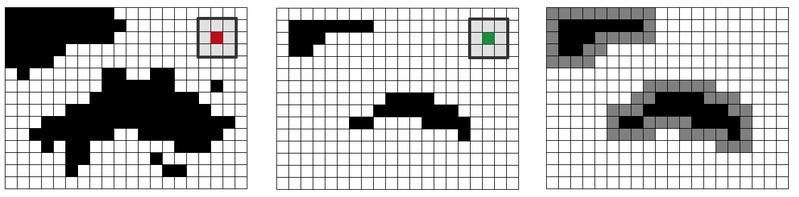
\includegraphics[width=400px]{otwarcie_przyklad.png}
            \caption{(\textit{Źródło: https://pl.wikipedia.org}) Przykład z elementem strukturalnym \(3 \times 3\) z punktem centralnym na środku.
            Jak możemy zauważyć, pojedyncze piksele (nie posiadające sąsiadów z wartością 1 zostały usunięte. Następnie reszta obiektów zostaje odbudowana.}
        \end{figure}
        \subsection{Zamknięcie morfologiczne}
        {
            \Large
            \justifying
            \quad
            Zamknięcie morfologiczne - jest równowazne dwóch następujących po sobie operacjach na obrazie: dylatacji, a następnie erozji.
            Wykonanie dylatacji, a następnie erozji pozwala nam zamknąć niektóre obiekty, a następnie przywrócić pozostałe obiekty do stanu sprzed dylatacji.
        }
        \begin{figure}[H]
            \centering
            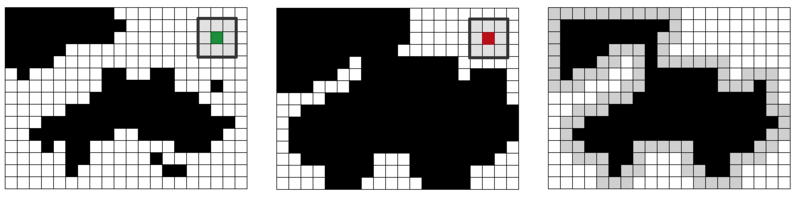
\includegraphics[width=400px]{zamkniecie_przyklad.png}
            \caption{(\textit{Źródło: https://pl.wikipedia.org}) Przykład z elementem strukturalnym \(3 \times 3\) z punktem centralnym na środku.
            Jak możemy zauważyć, piskele, które wcześniej były odłączone od wiekszego obiektu ale leżały niedaleko teraz stanowią integralną jego cześć,
            a dwa większe obiekty połączyły się.}
        \end{figure}
        \subsection{Korekcja Gamma}
        {
            \Large
            \justifying
            \quad
            Korekcja Gamma - operacja punktowa wykonywana na obrazie monochromatycznym, które bazuje na krzywej gamma i wyraża się ją za pomocą wzoru \(L'(x,y) = L(x,y)^\gamma\)
            Zastosowanie \(\gamma = 1\) sprawia, że nic się nie zmieni.
            Natomiast w przypadku, gdy \(\gamma > 1\) obraz zostanie przyciemniony.
            Analogicznie gdy \(\gamma < 1\) obraz zostanie rozjaśniony, rzy czym założeniem jest: \(\gamma \epsilon \left[0,1\right]\).
        }        
        \begin{figure}[H]
            \centering
            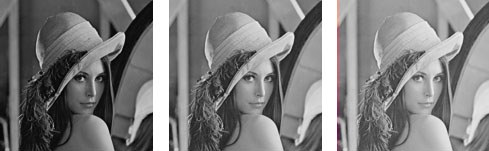
\includegraphics[width=400px,height=120px]{korekcja_gamma_przyklad.jpg}
            \caption{(\textit{Źródło: http://www.algorytm.org}) Od lewej: \(\gamma > 1\) obraz przyciemniony, \(\gamma = 1\) brak zmian, \(\gamma < 1\) obraz zostaje rozjasniony.}
        \end{figure}
    \newpage
    \section{Część Praktyczna}
        \subsection{Wykorzystane oprogramowanie}
        \subsection{Diagram UML aplikacji}
        \subsection{Omówienie implementacji}
        \subsection{Omówienie interfejsu}
        \subsection{Listing kodu}
    \newpage
    \section{Wyniki}
    \section{Wnioski}
    \newpage
    \section{Podsumowanie}
    \newpage
    \section{Bibliografia}
    \begin{thebibliography}{9}
        \bibitem{digitalimageprocessing}
        Rafael C. Gonzalez and Richard E. Woods
        \textit{Digital Image Processing Third Edition}
        \bibitem{encyclopediaofgraphicsfileformats}
        Murray, James D; VanRyper, William
        \textit{Encyclopedia of graphics file formats}
        \bibitem{whatisrequriedforgoodadhesion}
        Susanna Laurén
        \textit{What is required for good adhesion?}
        \url{https://www.biolinscientific.com/blog/what-is-required-for-good-adhesion}
        \bibitem{aipocwiki}
        \textit{Cyforwe przetwarzanie obrazów binarnych}
        \url{https://pl.wikipedia.org/wiki/Cyfrowe_przetwarzanie_obraz%C3%B3w_binarnych}
        \bibitem{tiffwiki}
        \textit{TIFF}
        \url{https://en.wikipedia.org/wiki/TIFF}
        \bibitem{gammacor}
        \textit{Korekcja gamma}
        \url{http://www.algorytm.org/przetwarzanie-obrazow/korekcja-gamma.html}
        \bibitem{msdocsmsbuild}
        Microsoft Docs
        \textit{MSBuild}
        \url{https://docs.microsoft.com/en-us/visualstudio/msbuild/msbuild?view=vs-2019}
        11/04/2016
    \end{thebibliography}
    \newpage
    \listoffigures
\end{document}